\chapter{System Overview}

\cref{fig:lorna_setup} shows the high level architecture of the LORNA concept. 

The xVIO state estimator uses the camera, IMU and laser range finder sensor onboard the vehicle in order to estimate the current state of the rotorcraft at any given time. Using map based localization (MBL) on HiRISE satellite maps allows for global localization. These poses are given to the flight controller and the output from that internal estimator is fed to the autonomy as well as the landing site detection nodes.

As mentioned above, the rotorcraft is flown using a PX4 flight controller. It communicates with the autonomy framework using the MAVROS ROS wrapper for the MAVLink rotorcraft protocol. This connection is used for the transmission of waypoint information and the setting of parameters.

The sensor images and their respective associated drone pose are given the landing site pipeline. In a first step, the 3D terrain is reconstructed using a structure from motion node. The reconstructed terrain is then given to the landing site detection algorithm(LSD) which first aggregates the information in a robot-centric multi resolution depth map and then segments valid landing sites on that. Detected landing sites are given to the autonomy to make the required adaptive landing decisions.



\begin{figure}[ht]
    \centering
    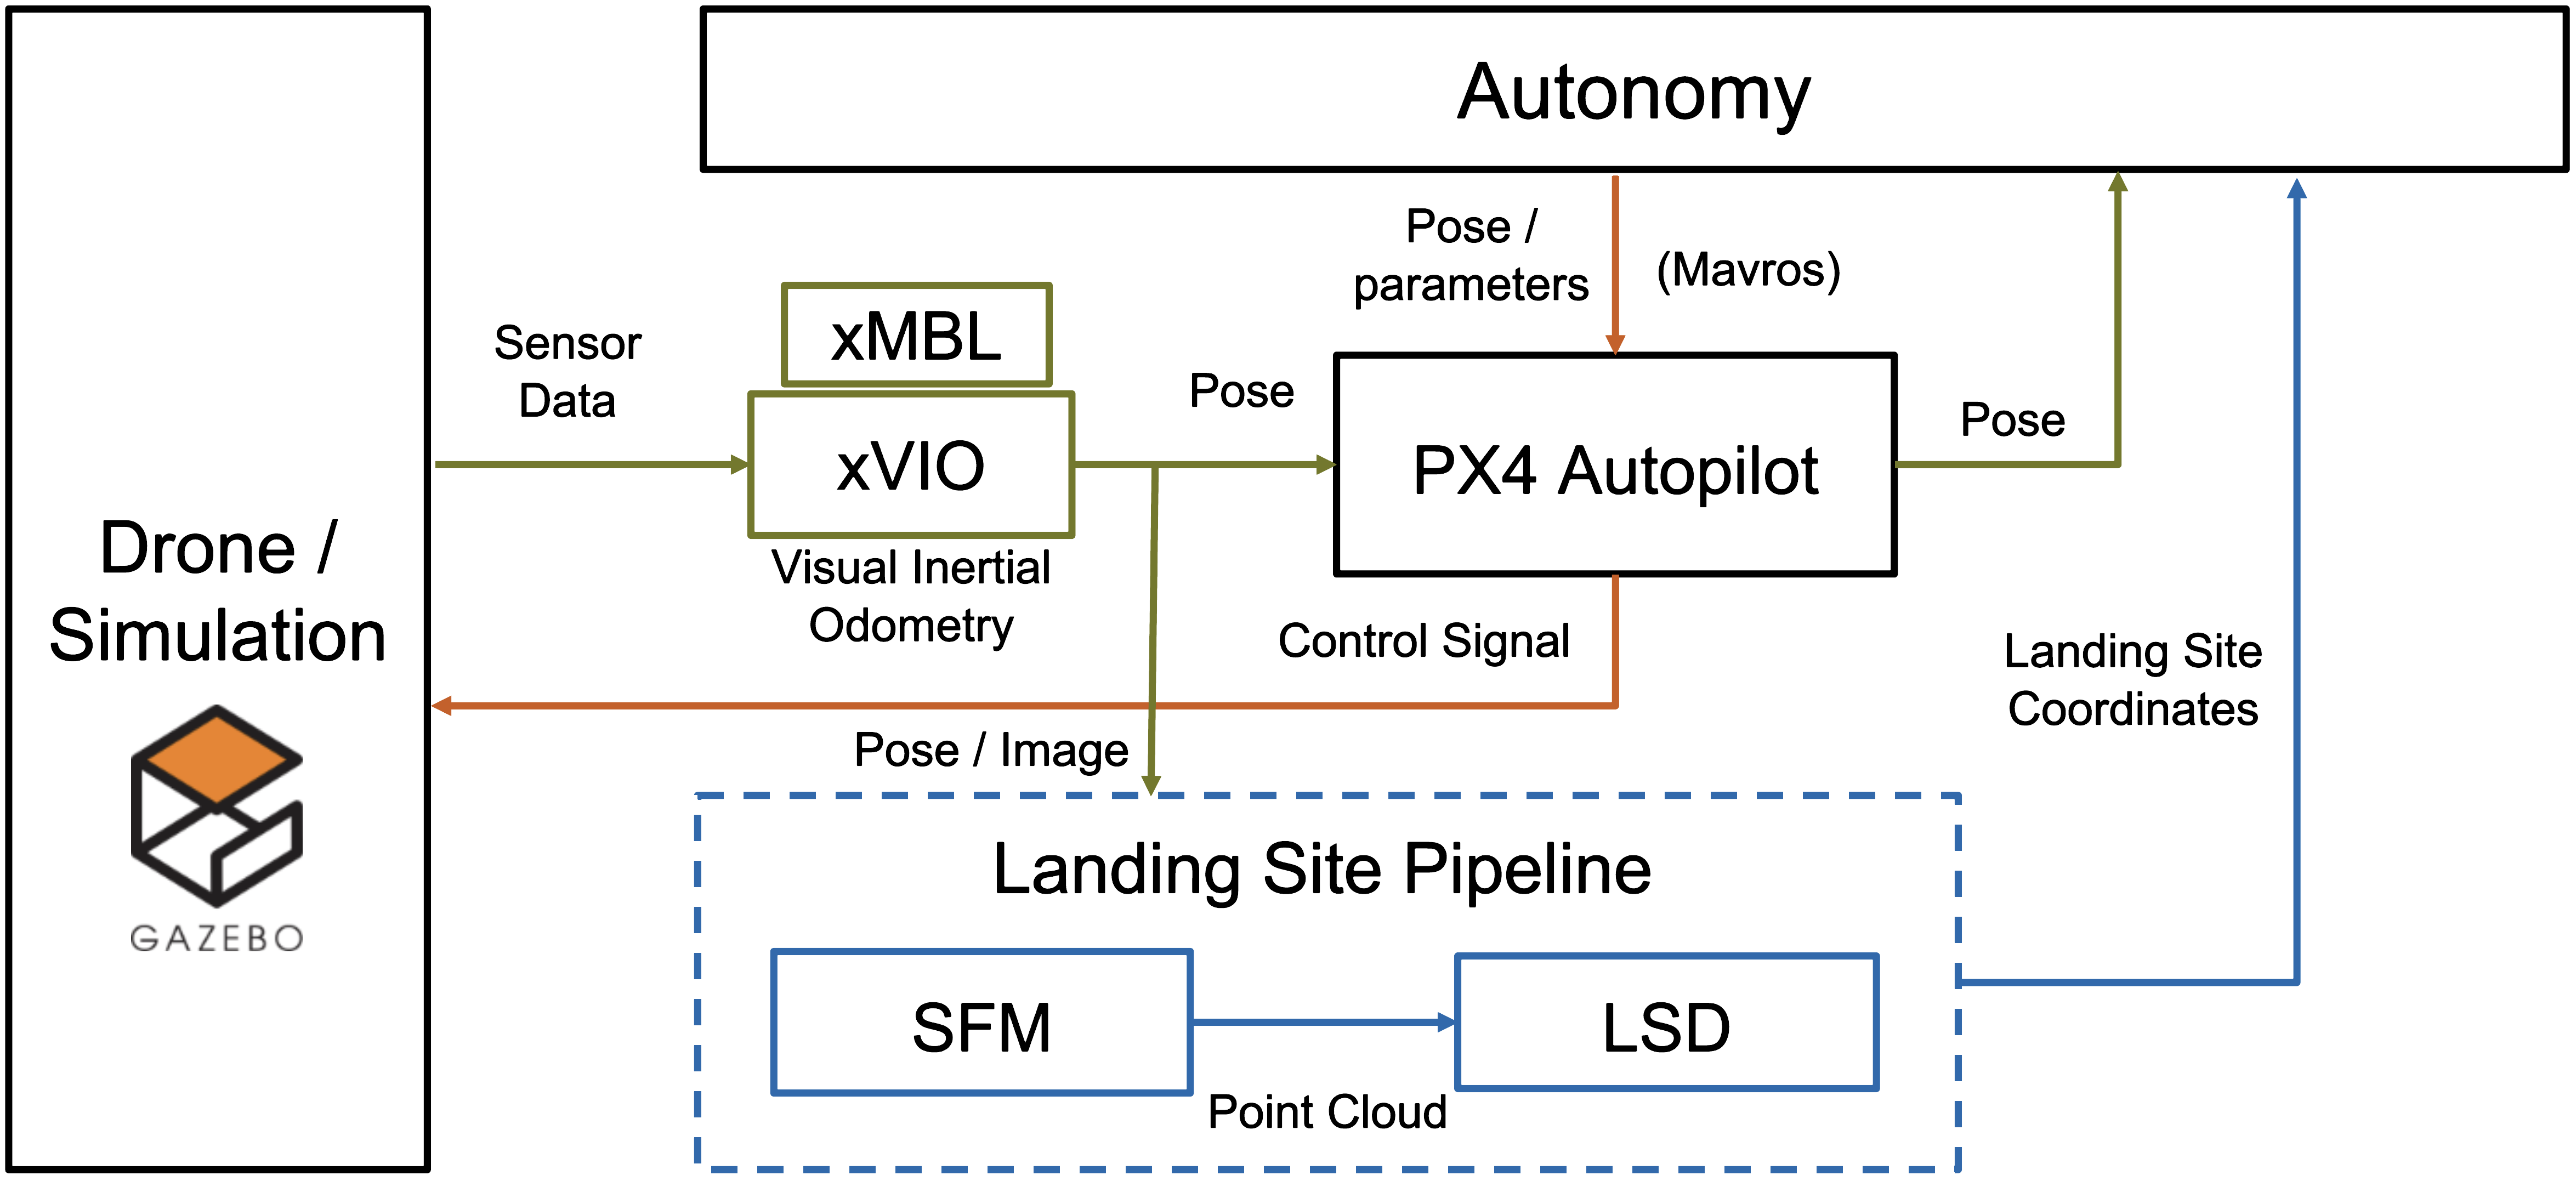
\includegraphics[scale=0.18]{images/system_overview/setup_flowchart_with_vio.png}
    \caption{LORNA Project Setup}
    \label{fig:lorna_setup}
\end{figure}

As the state estimator and the map based localization were not fully implemented at the time of this work, ground truth pose information from the simulated sensors was used instead. This is shown in \cref{fig:lorna_setup_GT_pose}

\begin{figure}[ht]
    \centering
    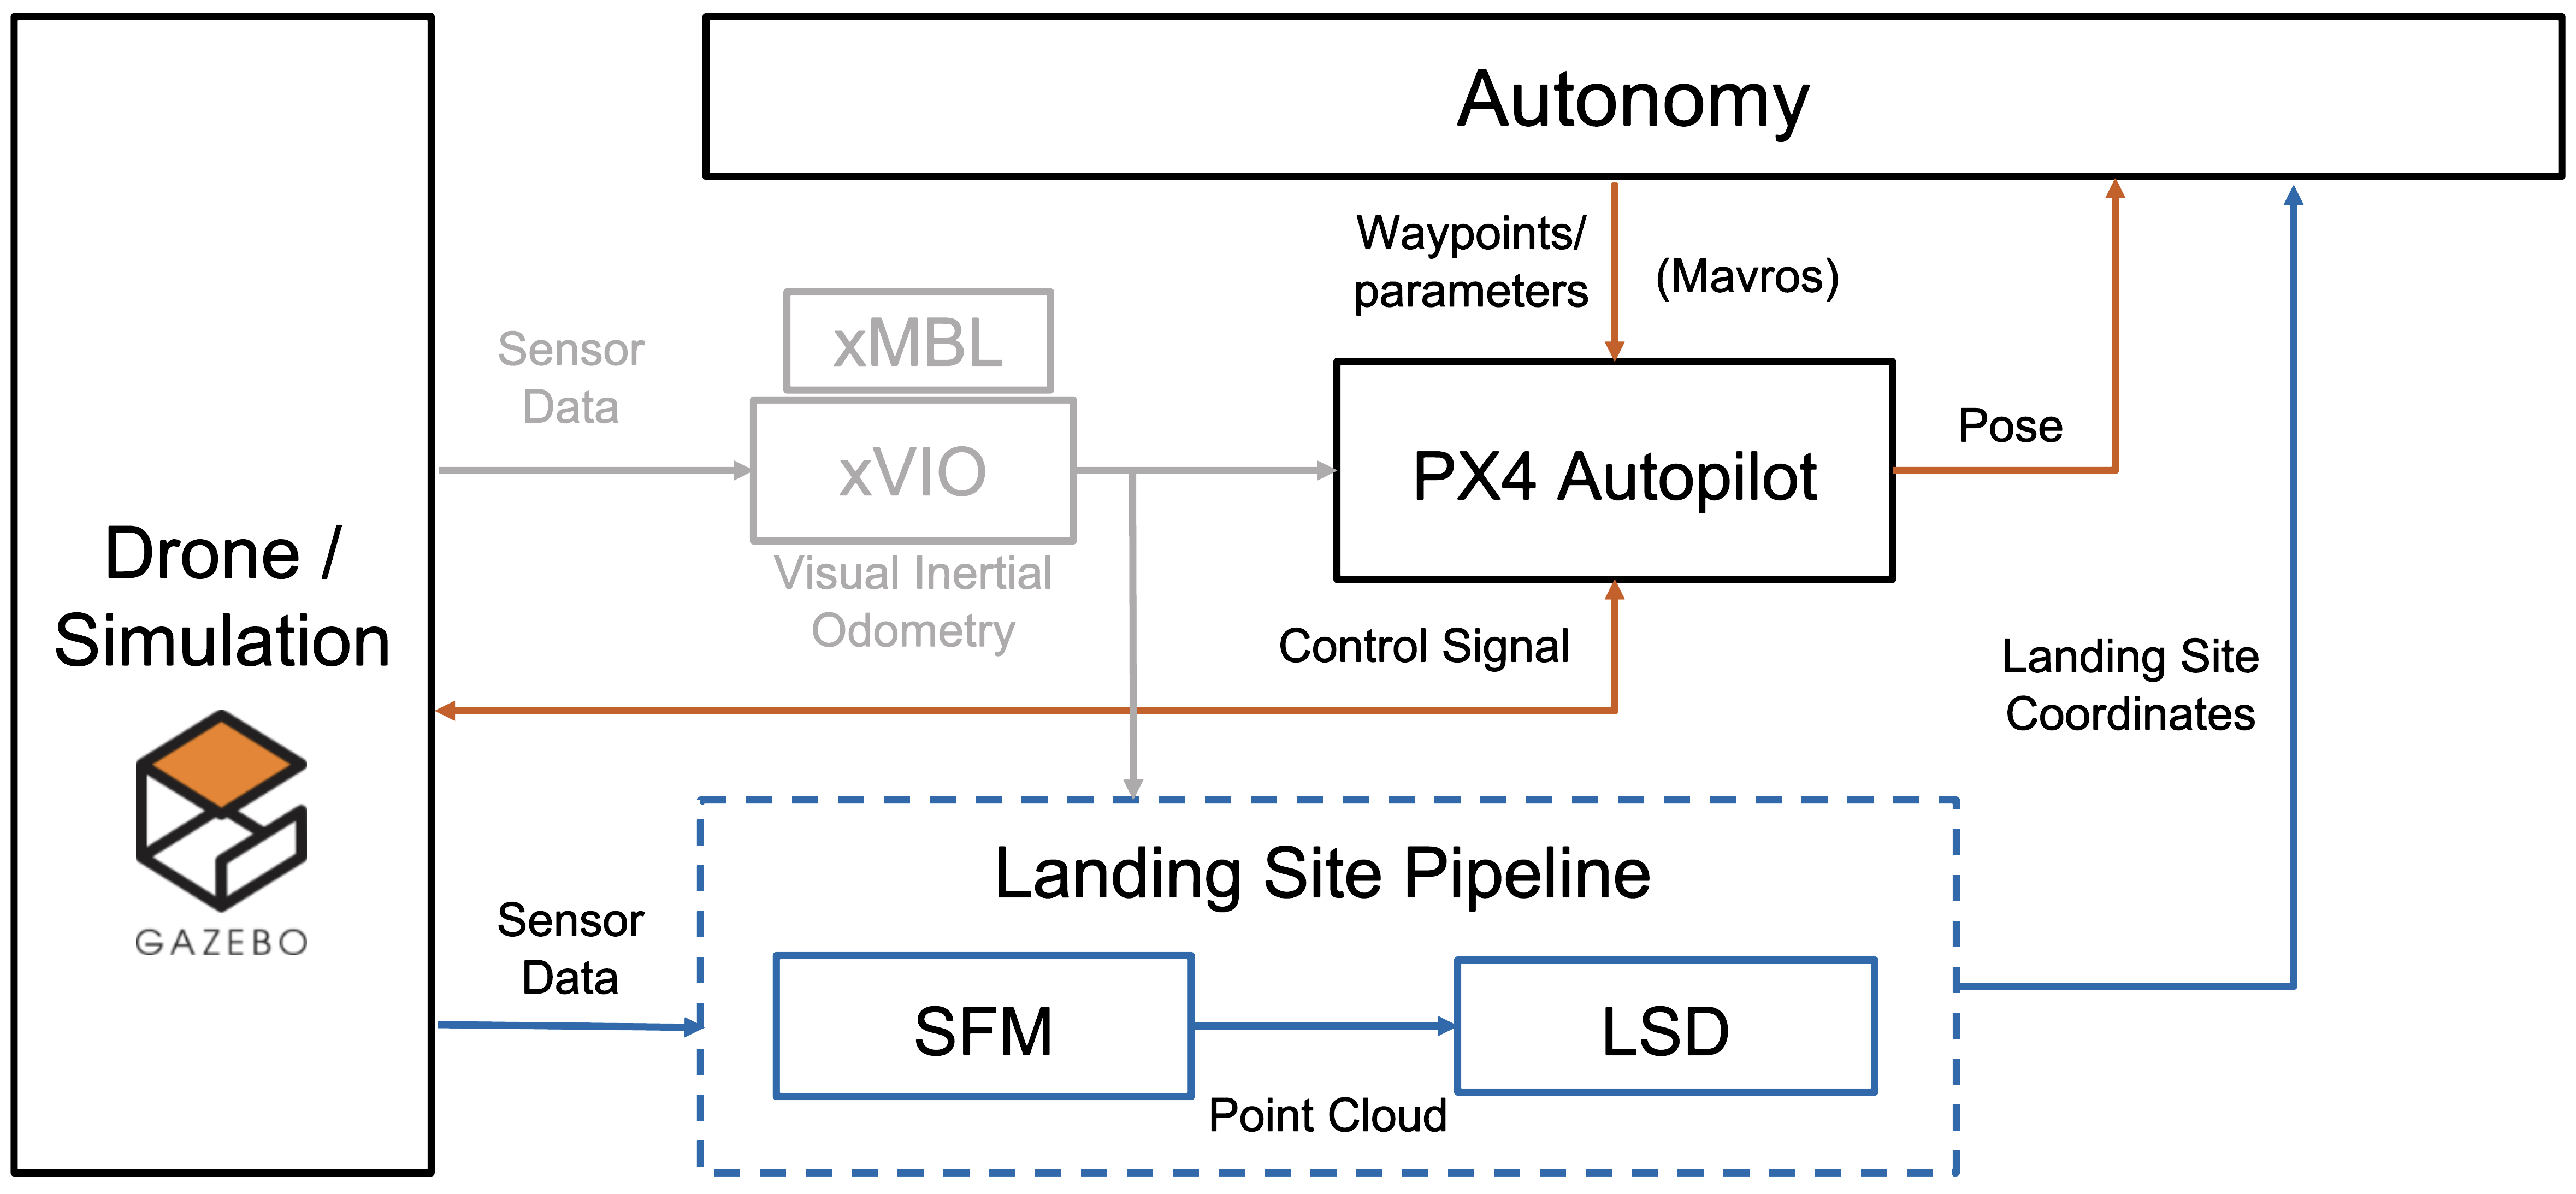
\includegraphics[scale=0.18]{images/system_overview/setup_flowchart.png}
    \caption{LORNA Project Setup with GT pose}
    \label{fig:lorna_setup_GT_pose}
\end{figure}

Since this thesis focuses on the integration of existing software instances, it is essential to delve into each component and elucidate their operational mechanisms.

\clearpage %HERE
\section{Simulation}

In this work I almost exclusively used a drone simulation. This allowed for a facilitated development with respect to both speed and safety. The choice of simulator, which is Gazebo Garden, was made prior to this work during the development of the autonomy.

\begin{figure}[ht!]
    \centering
    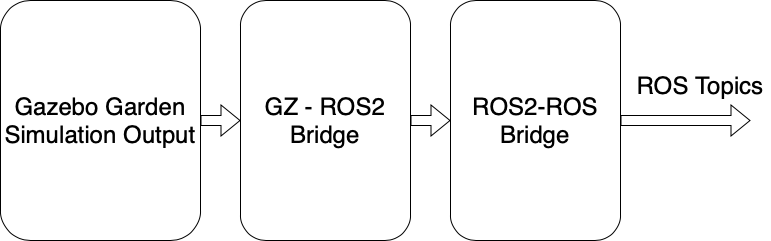
\includegraphics[scale=0.45]{images/system_overview/GZ_flowchart.png}
    \caption{Gazebo ROS Bridge}
\end{figure}


As the entire software stack of the LORNA project is dependent on ROS instead of ROS2, a bridge was used to convert the sensor information from Gazebo to ROS2 and from ROS2 to a ROS topic.


\section{Landing Site Detection Pipeline}\label{sec:setup:LSP}

The landing site detection pipeline consists of two nodes. A structure from motion node \citep{SFM} which creates a point cloud using a key frame based stereo depth approach on monocular images and a landing site detector algorithm \citep{LSD1, LSD2} which aggregates the depth measurements into a rolling buffer based multi-resolution depth map and segments landing sites on the created DEM. These found landing sites are then supplied to the autonomy. 

\subsection{Structure From Motion (SFM)}\label{subsec:setup:SFM}

The structure from motion approach retains images and their associated pose priors as key frames in a sliding window buffer. These key frames are used for a bundle adjustment pose refinement and subsequently, using a previously stored key frame and the incoming pair, a stereo depth algorithm is applied to achieve a depth image. 

In the following, the three main parts are explained in more detail:

\subsubsection{Key Frame Handling}

At the end of an iteration the key frames are updated. Naturally, in the beginning before the rolling buffer is filled, each incoming frame is simply added to the back of the buffer queue. Upon reaching the queue's maximum capacity, incoming frames are analyzed regarding the two following factors:

\begin{itemize}
    \item \textbf{Frame to frame parallax}

    To ensure that enough distance has been covered between the last key frame and the incoming frame, the root-mean-square value for the parallax distance of the matched features is calculated and compared with a minimum threshold.
    \item \textbf{Information retention and contribution}

    To advance the buffer over time, new information should be added. Therefore, new features should be detected on an incoming image. To match the incoming image with the existing key frames however, sufficient features must also be shared with the previously detected key frames.
\end{itemize}

Therefore, if these two conditions are fulfilled, a new frame is accepted in the buffer. To determine the quality of the current key frames, the oldest key frame is used to determine the following metrics:

\begin{itemize}
    \item \textbf{Number of matched features between the two frames}
    \item \textbf{Overlap of the two image footprints}
    
    Using the simple pinhole model formula for an image footprint and the calculated baseline, the overlap of the areas are calculated.
    \item \textbf{Feature area ratio}
    
    The maximum rectangle spanning all features is derived for both frames. Due to parallax from lateral motion, they don't overlap allowing to determine the area ratio of the feature span overlap.
\end{itemize}

If these three metrics lie above a certain threshold, the key frames are considered good and only the newest key frame is exchanged, retaining all others. If not, the new frame is added to the back, pushing the rolling buffer further, leading to the loss of the oldest previous key frame.

\subsubsection{Bundle Adjustment}

Before doing 3D reconstruction, the poses are refined using a bundle adjustment algorithm. This is beneficial as the state estimator will always come with a certain error which drifts over time. 

\begin{figure}[ht!]
    \centering
    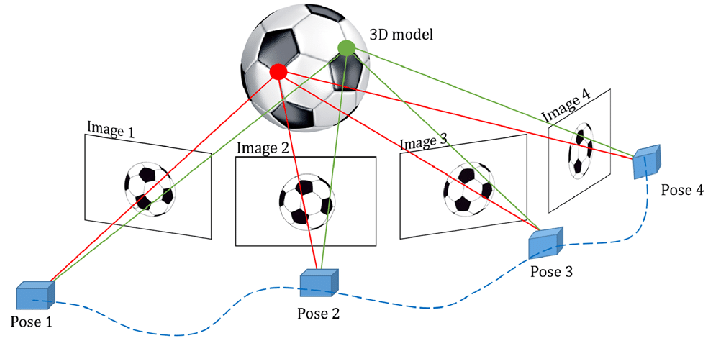
\includegraphics[scale=0.5]{images/system_overview/BA.png}
    \caption{Bundle Adjustment Procedure as shown in \citet{BA}}
    \label{fig:BA}
\end{figure}

\cref{fig:BA} shows the change in reprojection, which the bundle adjustment optimization technique thrives to diminish. Generally, it does so by considering a number of key frames and optimizing their poses as well as the camera parameters used to acquire the images. In this case, only the pose refinement is considered for the key frames in question.

\subsubsection{Stereo Depth}

Having chosen adequate key frames and refined their poses, the crucial step of 3D reconstruction can be performed. For this, the key frames are checked to have an image overlap with the new image that is sufficient but not fully overlapping and to have a small enough baseline inclination so that assuming the same altitude above ground is reasonable. If the checks are successful, the key frame with the largest baseline to the new frame is chosen for the stereo procedure. 

Using the two frames and the parallax distance between the detected features due to lateral motion between the images, the disparity values can be derived. With the camera's intrinsic parameters and the disparity values, a depth image of the terrain can be created. Then, using these depth values of the individual and the camera parameters, the 3D coordinates of each detected point can be calculated, and thus the depth image is converted into a point cloud which is the format required for LSD.

% TODO images of terrain and depth image created


\subsection{Landing Site Detection (LSD)}\label{subsec:setup:LSD}

\subsubsection{Depth Aggregation}\label{subsubsec:setup:aggregation}

\begin{figure}[ht!]
    \centering
    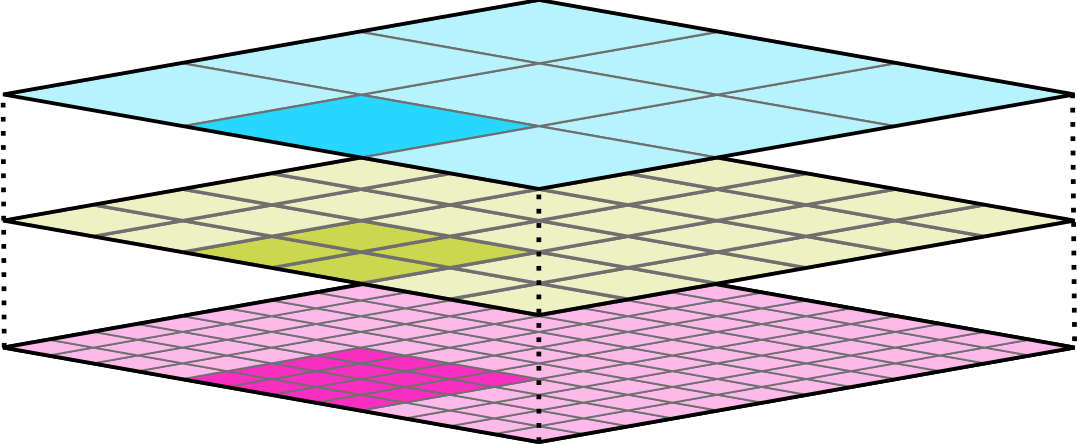
\includegraphics[scale=0.25]{images/system_overview/DEM.png}
    \caption{Multi Resolution Depth Map}
    \label{fig:DEM}
\end{figure}

The foundation of the landing site detection mechanism is a rolling buffer based multi resolution depth map as indicated in \cref{fig:DEM}. Each base layer cell is represented with 4 cells at a higher resolution layer.

Each point cloud input iteration, the measurements are placed in the respective cells based on the level of detail of the perceived points. In a subsequent step the measurements are pooled up and down the resolution layers in order to make the DEM more consistent and interpolate missing values.

Each cell in this dense elevation map (DEM) is comprised of an optimal mixture of gaussian (OMG) state as described in \citet{LSD2}.

Its update step looks like this:

\begin{align}
    S_t &= S_{t-1} + \sigma_{x_t}^{-2}\\
    \mu_t &=  \frac{1}{S_t}\left(S_{t-1}\mu_{t-1} + \frac{x_t}{\sigma_{x_t}^2}\right)\\
    \sigma_t^2 &=  \frac{1}{S_t}\left( S_{t-1}(\sigma_{t-1}^2 + \mu{t-1}^2) + \frac{x_t^2}{\sigma{x_t}^2} + 1 \right) - \mu_t^2
    \label{eq:OMG_updates}
\end{align}

Where $\mu_t$ is the cell's new mean value, $\sigma_t^2$ is the cell's variance and $S_t$ defines an auxilliary variable to keep track of all past variances within a single scalar.

Thus similar to Kalman filters, the OMG cells' uncertainties decline over time as more measurements are entered. Because of this the DEM's terrain estimate converges over time. 

\subsubsection{Hazard Segmentation}\label{subsubsec:setup:haz_seg}

On the created depth map landing sites can then be detected. This is done using a roughness and slope assessment of the perceived terrain. Roughness defines the maximum absolute altitude difference around a cell in a certain resolution layer and slope is determined by fitting a plane to the vicinity of a considered point.

If the roughness and slope values lie within the acceptance threshold, the spot is recognized as a landing site and marked as such in a binary landing map. 

\begin{figure}[ht!]
    \centering
    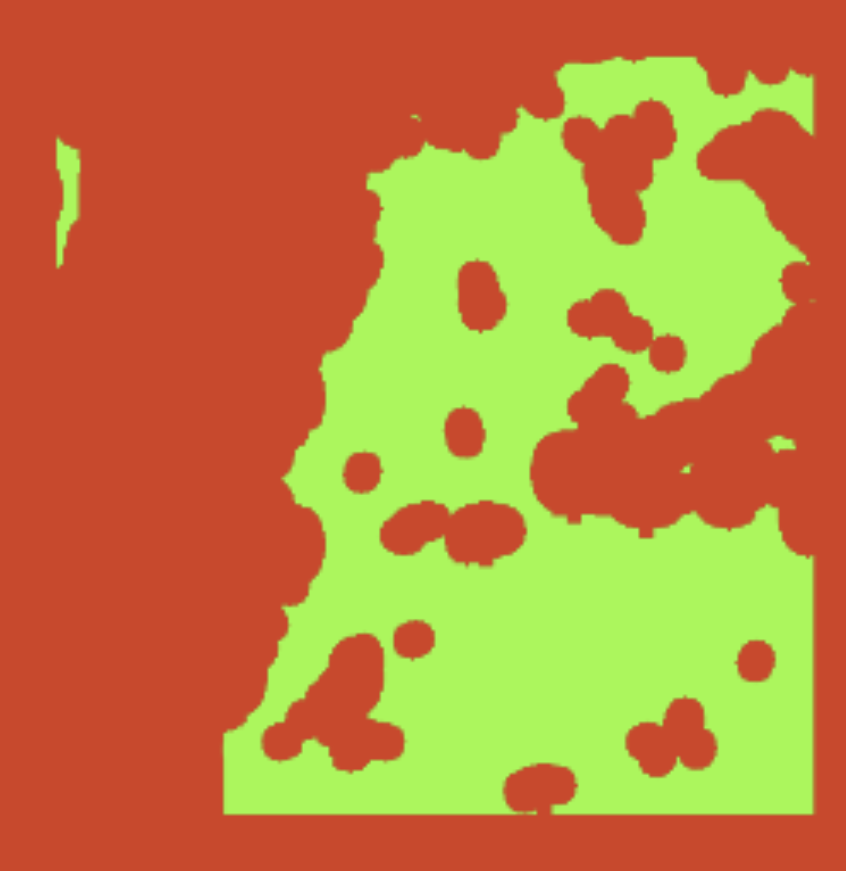
\includegraphics[scale=0.5]{images/system_overview/ls_map.png}
    \caption{Binary Landing Site Map}
    \label{fig:ls_map}
\end{figure}

\subsubsection{Landing Site Selection}\label{subsubsec:setup:ls_select}

After applying a distance transform on the landing site map and performing non-maximum suppression on the landing site sizes, the biggest landing sites are found. Their positions are then refined one last time using a mean shift algorithm that considers roughness, uncertainty and size once again. 

\begin{figure}[ht!]
    \centering
    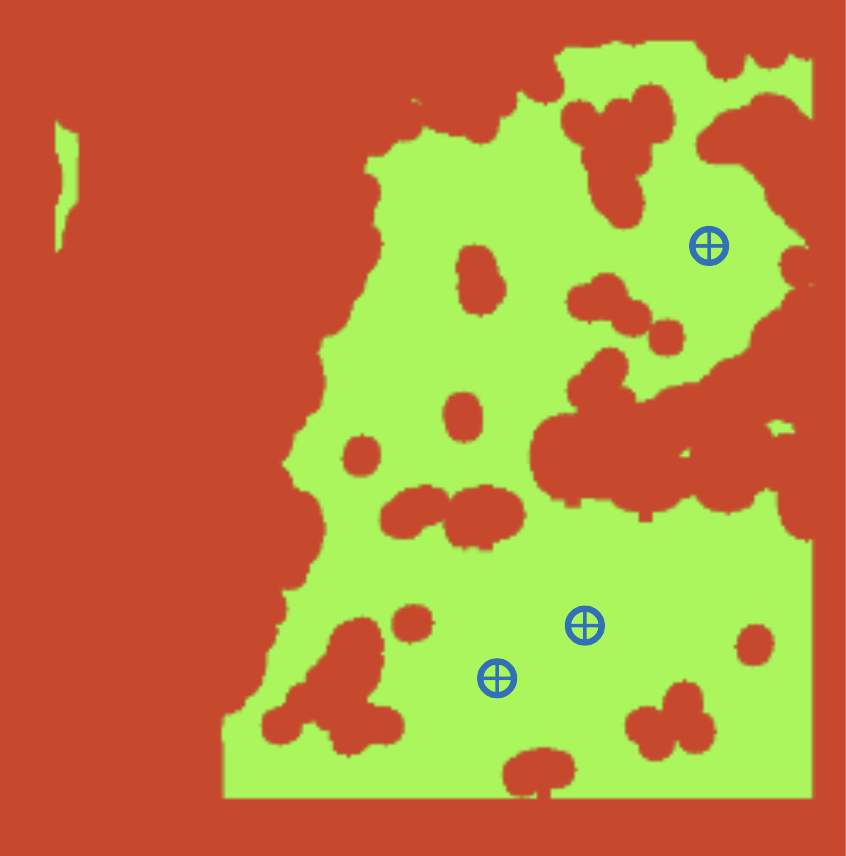
\includegraphics[scale=0.5]{images/system_overview/ls_map_nms.png}
    \caption{Binary Landing Site Map after Non Maximum Suppression}
    \label{fig:ls_map_nps}
\end{figure}

\clearpage %HERE

\subsubsection{Debug Images}

\begin{figure}[ht!]
    \centering
    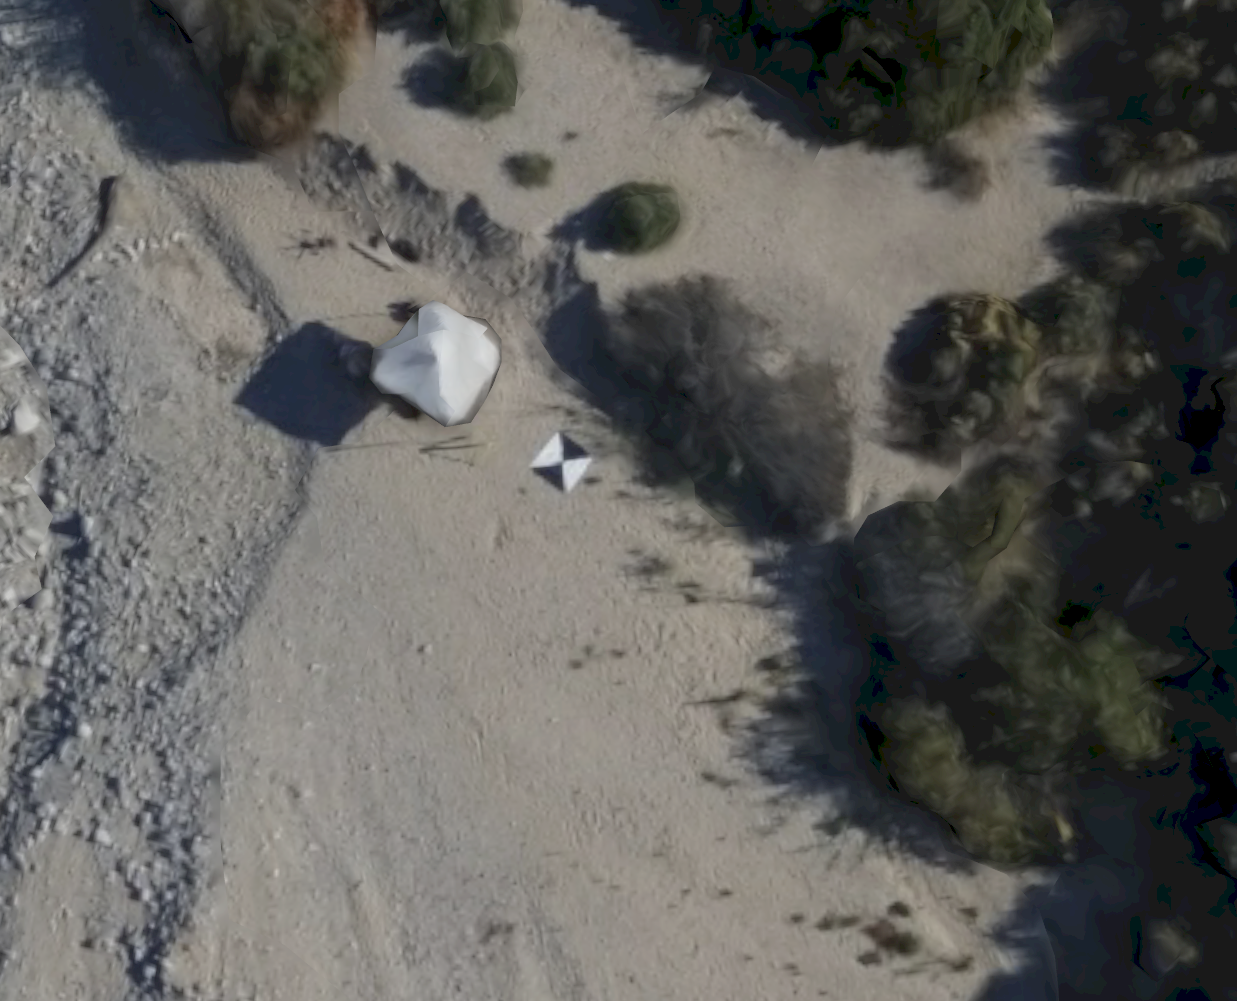
\includegraphics[scale=0.25]{images/system_overview/lsd_debug_reference.png}
    \caption{Gazebo Simulation Reference}
    \label{fig:lsd_debug_ref}
\end{figure}

\begin{figure}[ht!]
    \centering
    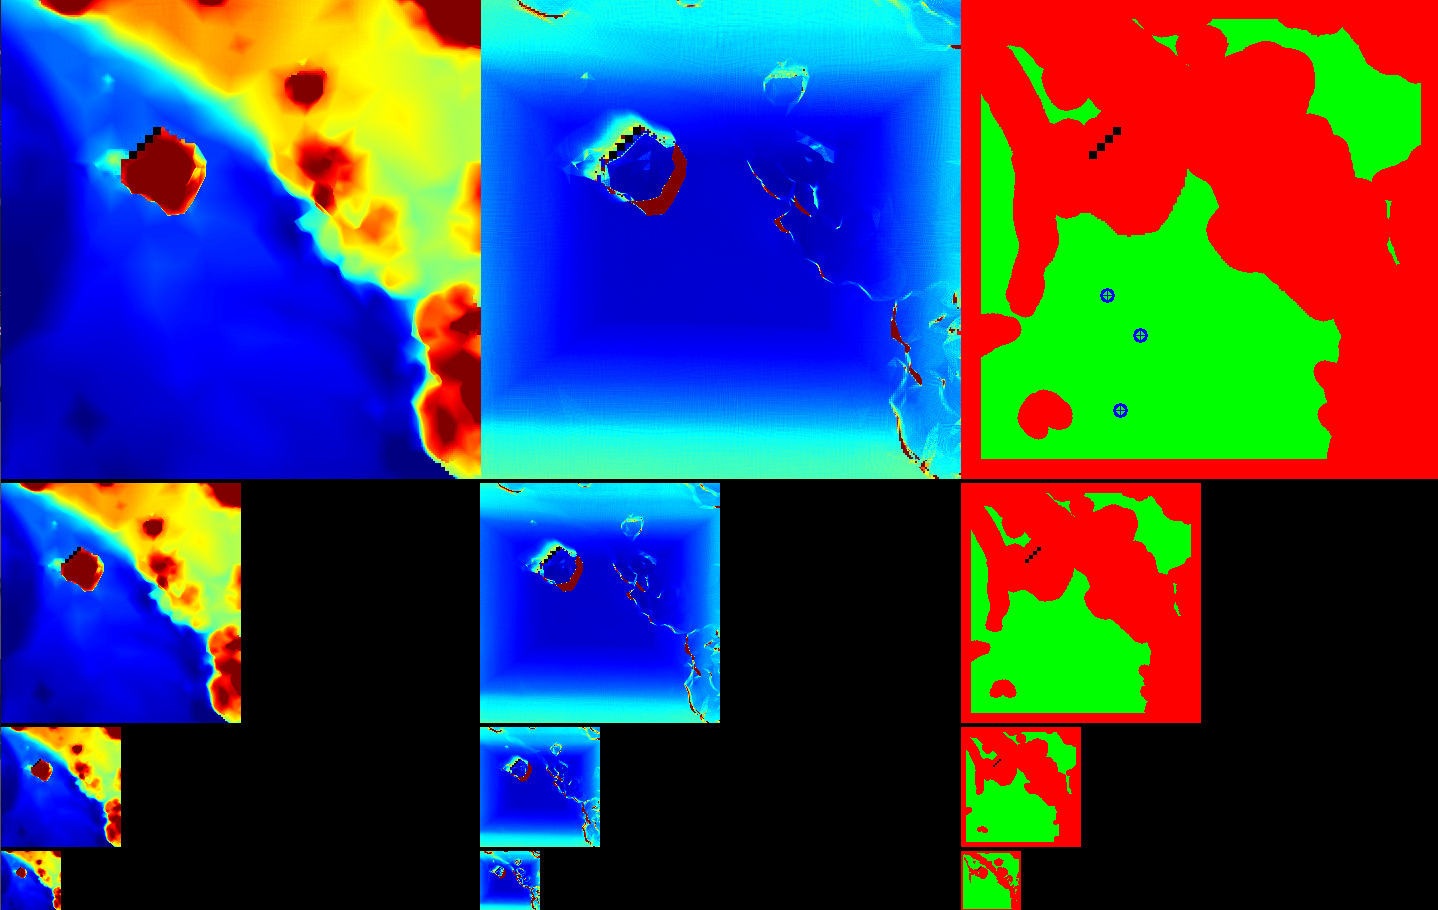
\includegraphics[scale=0.25]{images/system_overview/lsd_debug_image.png}
    \caption{LSD Debug Image - Left: DEM, Middle: Uncertainties, Right: LS Map}
    \label{fig:lsd_debug}
\end{figure}

The landing site detection debug image is a good comprehensive visualization of the landing spot detection procedure. 

On the left one can see the multi-resolution map displaying the same terrain area in different resolutions. Red pixels are closer, blue further away.

In the middle one can see the uncertainties of the detected points. For simplification purposes the variance of the detected points is simply the associated stereo depth error.

On the right is the above mentioned binary landing site map. Green indicates valid landing sites, and the blue crosses indicate the chosen non-max suppressed and mean shifted landing sites.

\section{Autonomy}\label{sec:setup:autonomy}

The autonomy framework was developed within the LORNA project. It is the overarching instance governing all the necessary behaviors and constituting the interface between all the different nodes of the process. It is connected to the flight controller through the Mavros wrapper of the Mavlink protocol. With this connection it can send waypoints and parameter updates to the flight controller.
In addition to the in \cref{fig:lorna_setup} shown connections it also communicates with a healthguard node keeping track of the systems health state and alerting in case of anomalies.

\begin{figure}[ht!]
    \centering
    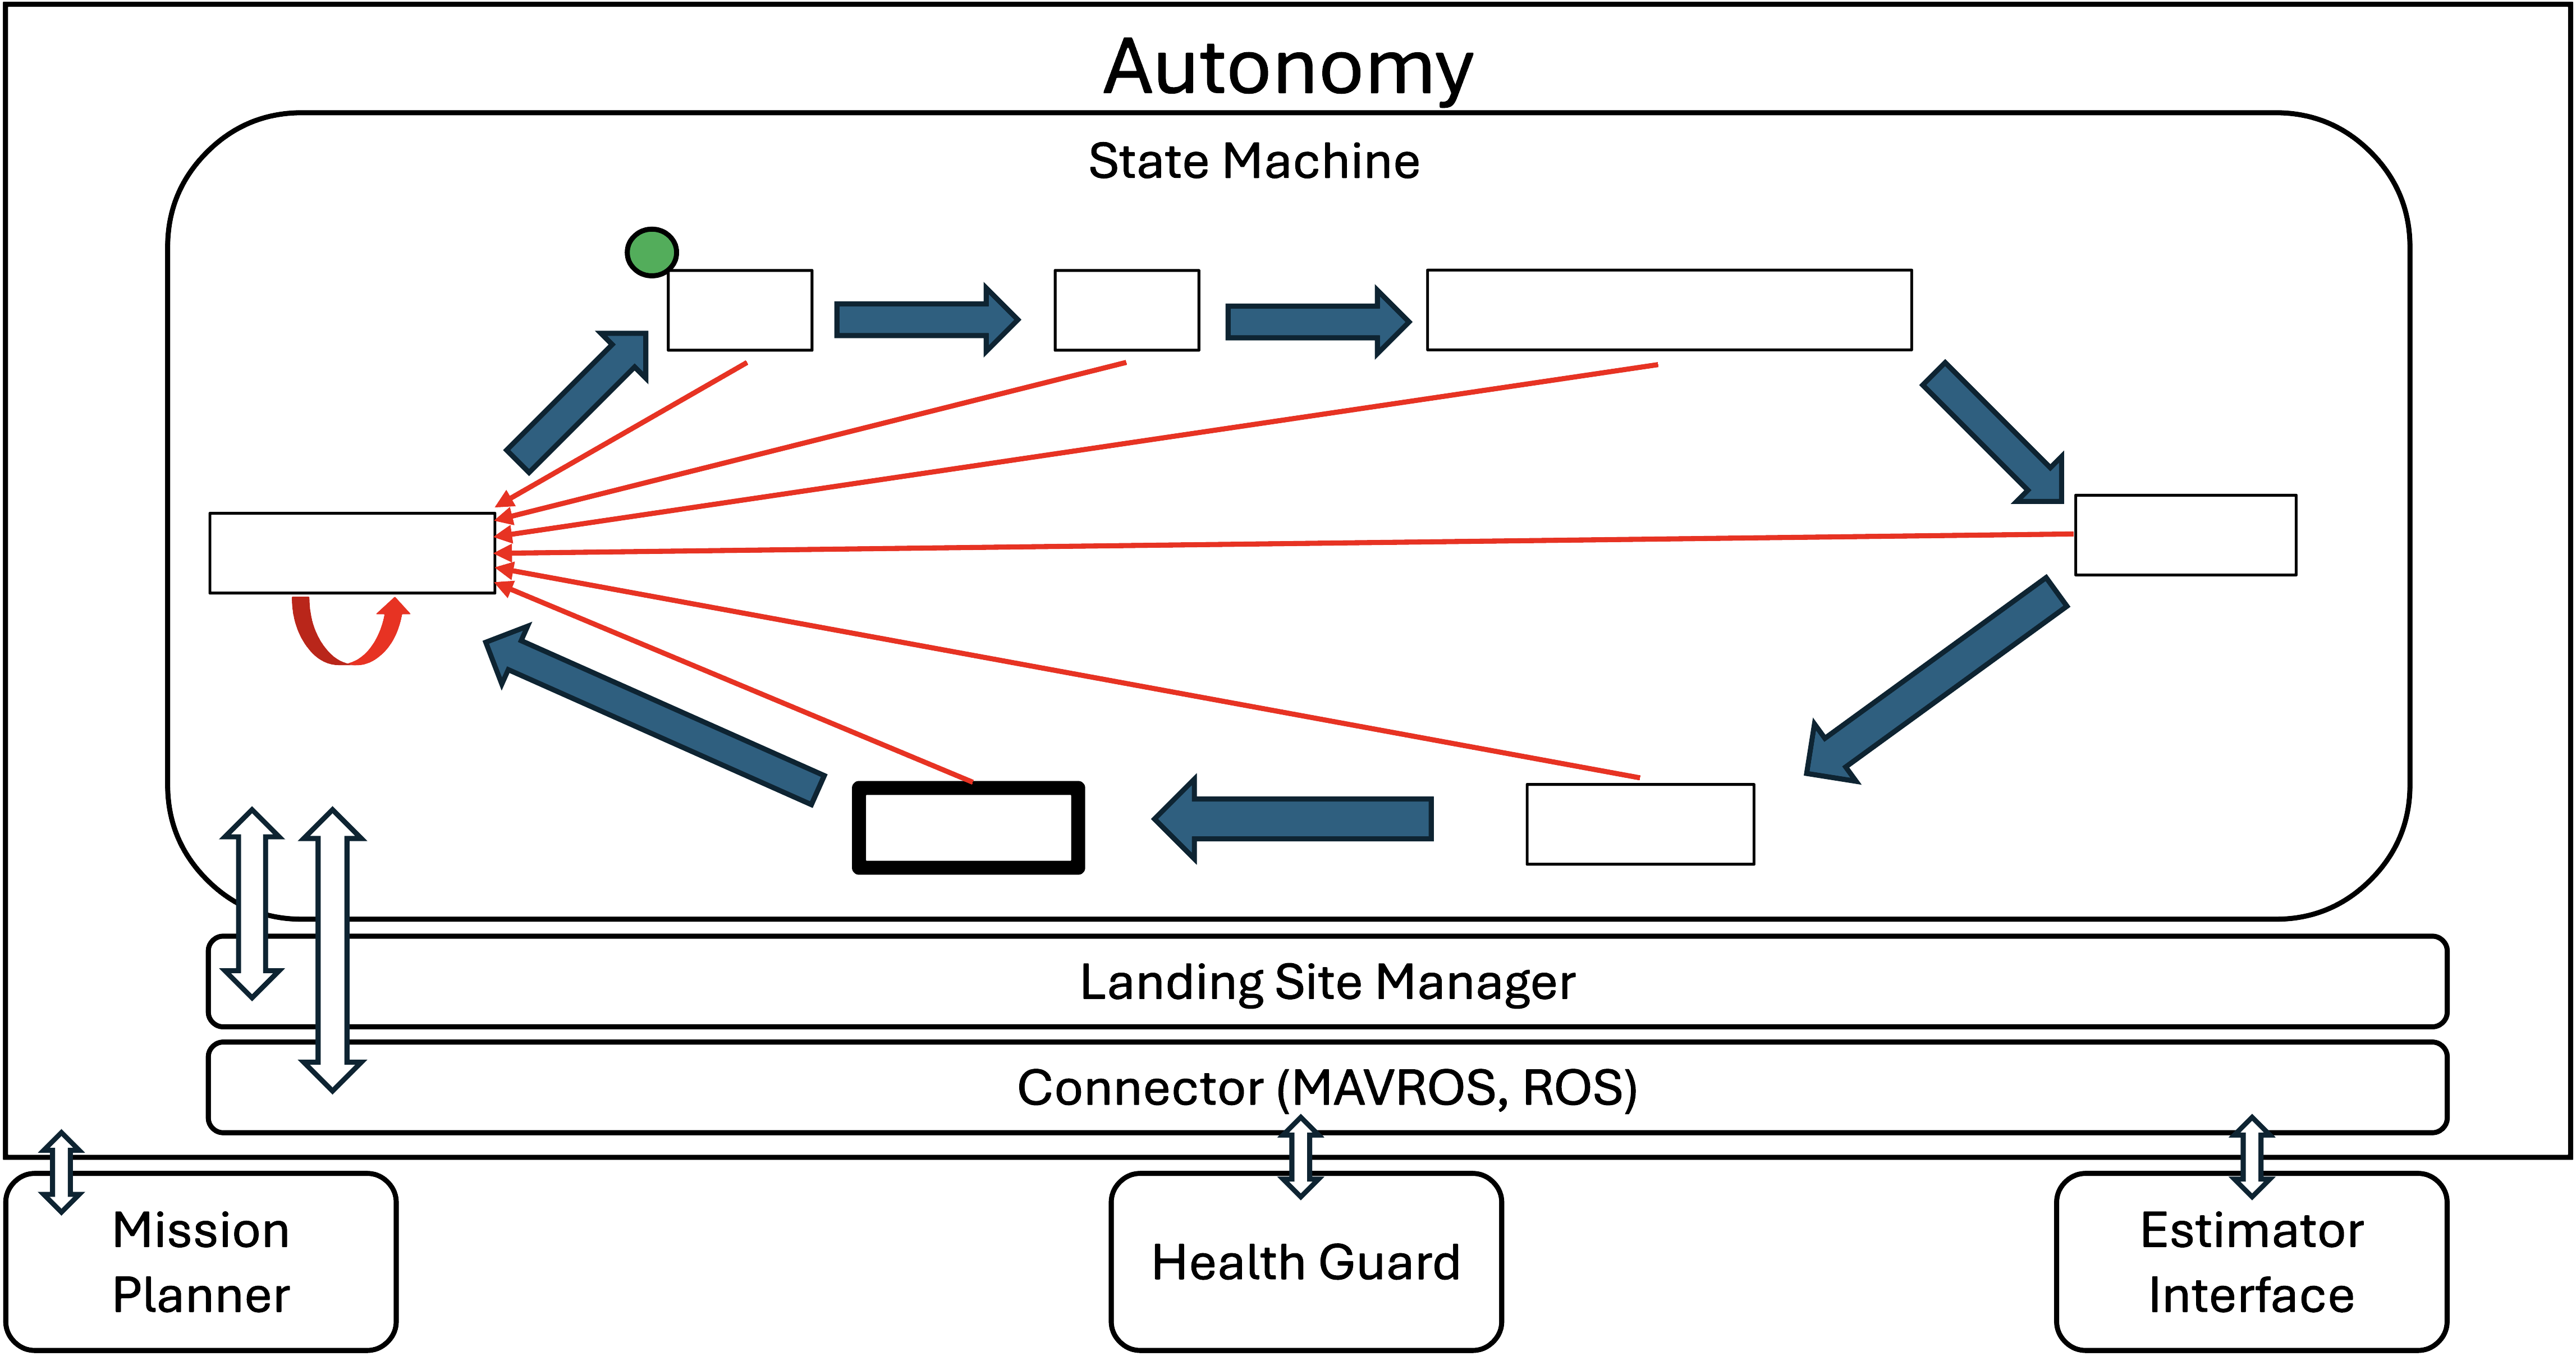
\includegraphics[scale=0.45]{images/system_overview/autonomy.png}
    \caption{Simplified Structure of the Autonomy}
    \label{fig:autonomy}
\end{figure}

The core of the autonomy is the state machine as depicted in \cref{fig:autonomy}. In each state the respective node is executed which most often is a single action node. For more complicated procedures a behavior tree is used. This is the case for the takeoff as well as the landing node. As indicated in bold, the landing node is the most crucial node in this work as this is where the landing behavior using the landing sites is executed.

In a separate process the landing site manager processes incoming landing sites. Prior to this work the landing site interface was a dummy implementation serving the framework's completeness.

The connector threads interact with the flight controller through Mavros and the other LORNA nodes through a ROS connector.

\subsection{Behavior Tree}\label{subsec:setup:behavior_tree}

The behavior tree framework within the autonomy is implemented in the traditional way, each comprised of a root node, control flow nodes and action nodes resulting in a modular structure enabling tasks of tremendous complexity. Additionally decorator nodes can be used which alter a single node and function as an add-on on the same level.

\subsubsection{Control Flow Nodes}

The most imported control flow nodes which were used in this thesis are the following:

\begin{itemize}
    \item \textbf{Fallback Node}: Attempts to execute first child node and if successfull returns a success state. Else it continues to the next child node. If no child node was successfull it returns the failure state. A boolean operator analogy for this would be the logical OR, stopping at the first successful entity.
    \item \textbf{Sequence Node}: Executes one child after another. It only returns the success state if all children nodes ran successfully. Otherwise it returns false. Here an analogy would be the logical AND boolean operator.
\end{itemize}

\subsubsection{Decorator Nodes}\label{subsubsec:decorator_nodes}

The most important decorator nodes are:

\begin{itemize}
    \item \textbf{Inverter Node}: Inverts the output of an action node. Boolean analogon would be the ! (not) operator.
    \item \textbf{Repeat Node}: Repeats a node a number of times until fails or a timeout is reached. 
    \item \textbf{Retry Node}: Similiar to the repeat node loop but it repeats the node a number of times only until it succeeds or a defined timeout is reached.
    \item \textbf{Timeout Node}: Adding a timeout to an action node which otherwise wouldn't be temporally limited.
\end{itemize}

\subsubsection{Action Nodes}\label{subsubsec:setup:action_nodes}

There are a multitude of actions required for the various subtask a rotorcraft has to perform during a mission. The most important ones for the landing behavior in this work are the following:

\begin{itemize}
    \item ChangeAltitudeAction: Changes the drone's altitude to the given value. The ascend / descend velocity diminishes upon reaching proximity to the desired waypoint.
    \item HoldPoseAction: Self-explanatory: the drone holds the current pose for a given time.
    \item LandingAction: Similar to the ChangeAltitudeAction, it descends to a waypoint which in this case is simply the ground vertically below the drone's current position. Upon reaching a certain proximity to the landing point, the descent velocity is reduced to a minimum in order to accomplish smooth landing.
    \item NavigateToWaypointAction: Lateral movement to the given waypoint. Same proximity based slow-down mechanism as ChangeAltitudeAction and LandingAction.
    \item RotateTowardsWaypointAction: Rotates the drone to face the given waypoint.
\end{itemize}








